\section{Algorithm Design}

% LCD, how to use order?


\begin{frame}
    \frametitle{Local Causal Discovery}
    % Generally (assumptions, set-up & method)

    \only<1>{
        Local Causal Discovery
        \begin{itemize}
            \item Local score-based method
            \item Given is some context variable $C$
            \item Test the presence of relations $X\to Y$
        \end{itemize}
    }
    
    \only<2>{
        Assumptions

        \begin{itemize}
            \item Structural Causal Model
            \item $C$ is exogenous
            \item Faithfulness
            \item Dependence and independence tests
            \item Unbiased data selection
            \item (Acyclicity)
        \end{itemize}
    }

    \only<3-4>{
        There is a relation $X\to Y$ if

        \begin{itemize}
            \item $C \CI Y \given X $
            \item $C \nCI Y$
            \item<4> \textcolor{gray}{$C \nCI X$}
            \item<4> \textcolor{gray}{$X \nCI Y$ }
            \item<4> \textcolor{gray}{$X \nCI Y \given C$ }
            \item<4> \textcolor{gray}{$C \nCI X \given Y$ }
        \end{itemize}
    }

    \only<5>{
        \begin{center}
            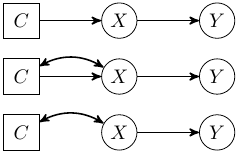
\includegraphics[width=.8\textwidth]{paper/5LCDgraphs}
        \end{center}
    }

    \only<6>{
        \begin{center}
            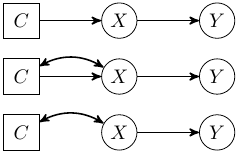
\includegraphics[width=.6\textwidth]{paper/5LCDgraphs}
        \end{center}

        \begin{itemize}
            \item $C$: is the data point interventional?
        \end{itemize}
    }

\end{frame}

\begin{frame}
    \frametitle{Order-Based LCD Outline}

    \only<1>{
        \begin{center}
            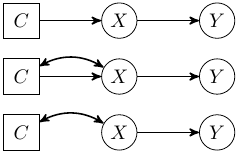
\includegraphics[width=.6\textwidth]{paper/5LCDgraphs}
        \end{center}

        \begin{itemize}
            \item Informing $C$ with \textbf{variable order} and \textbf{intervention target}
            \item Dependence between $C$ and $Y$ needs to go 'through' $X$
        \end{itemize}
    }

    \only<2>{
        \begin{center}
            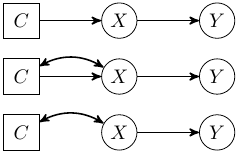
\includegraphics[width=.6\textwidth]{paper/5LCDgraphs}
        \end{center}

        \begin{itemize}
            \item $C$: did the intervention happen at, or 'before' $X$?
        \end{itemize}
    }

    \only<3>{
        \begin{enumerate}
            \item \textbf{Order inference}: find an ancestral order of train variables
            \item \textbf{Position estimation}: find the position of a test variable in that order
            \item \textbf{Causal inference}: use LCD with an order-based $C$ to test causal relations
        \end{enumerate}
    }

\end{frame}

% Modeling the order problem: MFAS is super hard, optimize penalty ratio (visual expl.), then estimate position in order

\begin{frame}
    \frametitle{Order Inference Task}

    \only<1>{
        Modeling the task

        \begin{itemize}
            \item Useful data: square intervention table
            \item Minimum Feedback Arc Set problem
            \item MFAS is Unique-Games hard
            \item Heuristic methods
        \end{itemize}
    }

    \only<2>{
        \begin{center}
            \huge $$\min_\pi p(\pi)$$
            $$p(\pi) = \frac{\sum_{\pi_i < \pi_j}|X_{ij}|}{\frac{1}{2}N(N-1)}$$
        \end{center}
    }

    \only<3>{
        \begin{center}
            {\huge $$\min_\pi r(\pi)$$}
            
            \large $$r(\pi) = \frac{\sum_{\pi_i < \pi_j}|X_{ij}|}{\frac{1}{2}N(N-1)} \frac{N(N-1)}{\sum_{i \neq j}|X_{ij}|} = \frac{2 \sum_{\pi_i < \pi_j}|X_{ij}|}{\sum_{i \neq j}|X_{ij}|}$$
        \end{center}
    }

    \only<4>{
        \begin{center}
            \includegraphics[height=.8\textheight]{3order/ordered_data_rand}
        \end{center}
    }

    \only<5>{
        \begin{center}
            \includegraphics[height=.8\textheight]{3order/ordered_data_good}
        \end{center}
    }

\end{frame}

% Approaches (focus: TS, SA, PR)
\begin{frame}
    \frametitle{Order Inference Experiments}

    \only<1>{
        Using the continuous intervention table
        \begin{itemize}
            \item Evolution Strategy: directly optimize ratio
            \item Edmonds algorithm: spanning arborescence of maximum weight
        \end{itemize}
    }

    \only<2>{
        Using the discretized intervention table
        \begin{itemize}
            \item Evolution Strategy: optimize binarized ratio
            \item TrueSkill, Social Agony, PageRank: scoring nodes and sorting
            \item Sun's algorithm: scoring nodes and breaking cycles
        \end{itemize}
    }

    \only<3>{
        \begin{itemize}
            \item TrueSkill
                \begin{itemize}
                    \item Video game skill level based on match outcomes
                    \item How likely is the gene an effect of some other genes with high certainty?
                \end{itemize}
            \item Social Agony
                \begin{itemize}
                    \item Hierarchy on directed social media
                    \item Agony is a penalty for being affected by a potential effect gene further down in the order
                \end{itemize}
            \item PageRank
                \begin{itemize}
                    \item Importance of webpages based on hyperlinks
                    \item How likely was a random effect caused by an intervention on this gene?
                \end{itemize}
        \end{itemize}
    }

    \only<4>{
        TrueSkill
        \begin{itemize}
            \item Matches encoded in a factor graph
            \item Sum-product algorithm yields mean and variance of each player's skill variable
            \item Score of 'player' $i$: $\mu_i-3\sigma_i$
        \end{itemize}
    }

    \only<5>{
        \begin{center}
            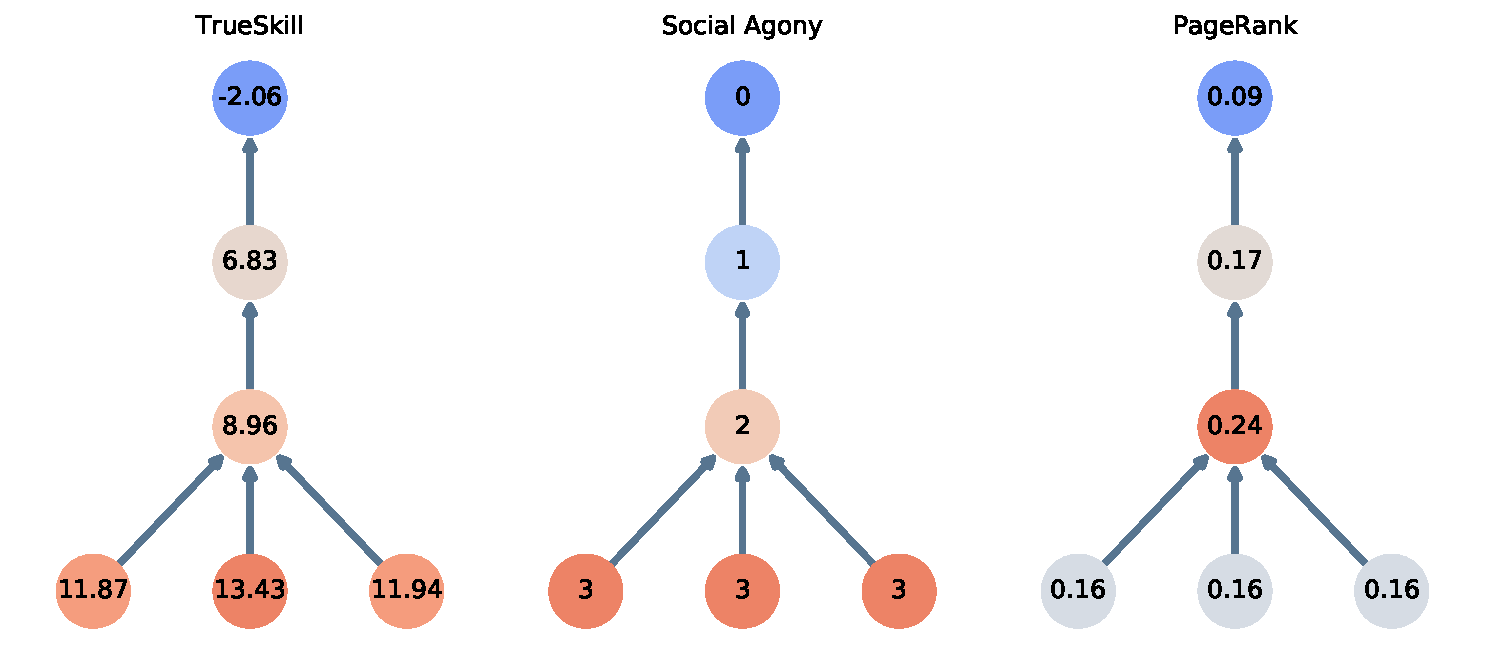
\includegraphics[width=\textwidth]{paper/4score_examples}
        \end{center}
    }
\end{frame}


% Results: TS best option, TS vs (SA,PR)
\begin{frame}
    \frametitle{Choice of Order Inference Method}

    \only<1>{
        \begin{center}
            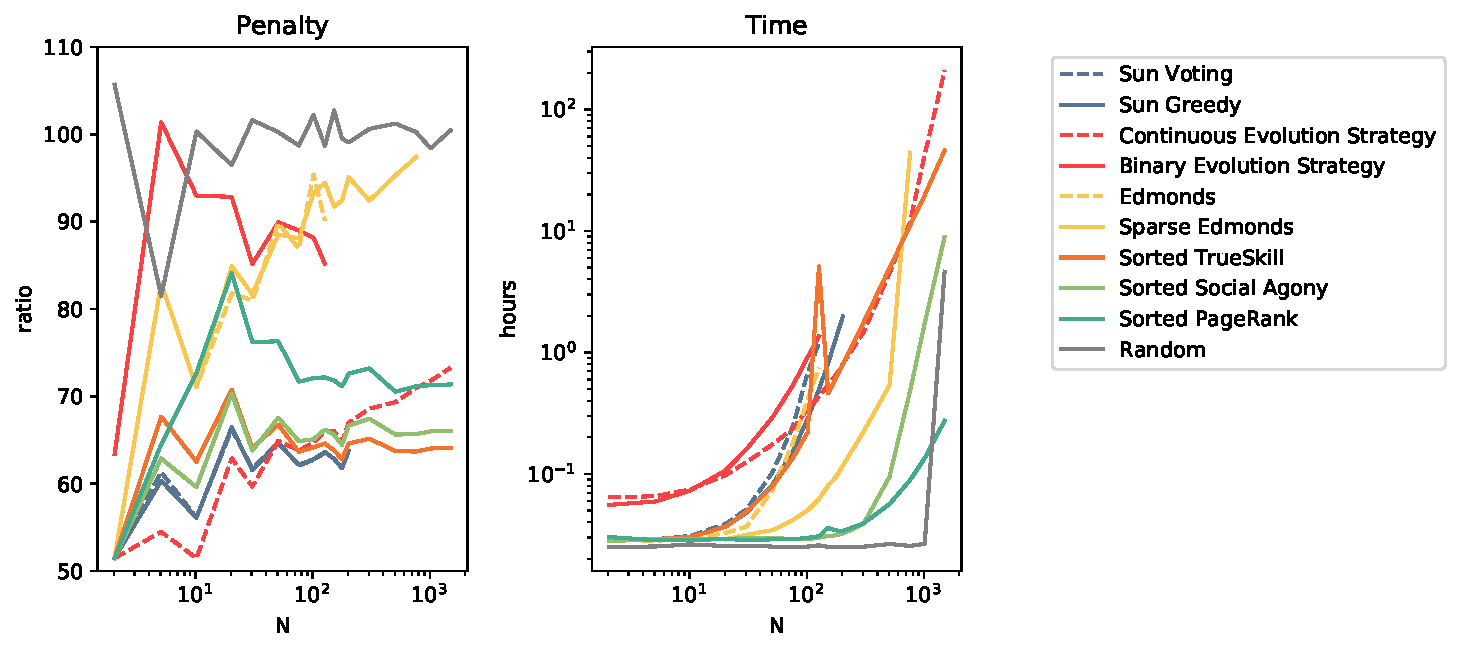
\includegraphics[width=\textwidth]{paper/4algorithm_global_comparison.pdf}
        \end{center}
    }

    \only<2>{
        \begin{center}
            \includegraphics[width=\textwidth]{3order/order_consistency}
        \end{center}
    }

    \only<3>{
        \begin{center}
            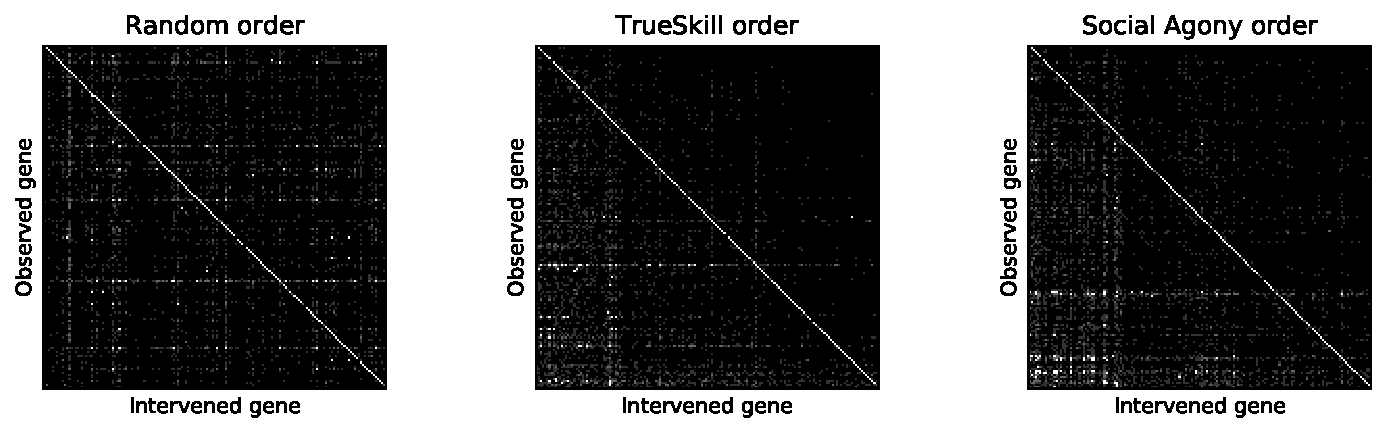
\includegraphics[width=\textwidth]{paper/4ordered_data}
        \end{center}
    }

    \only<4>{
        \begin{center}
            \includegraphics[height=.8\textheight]{3order/ordered_data_ts}
        \end{center}
    }

    \only<5>{
        \begin{center}
            \includegraphics[height=.8\textheight]{3order/ordered_data_sa}
        \end{center}
    }

\end{frame}    


% Estimating position in order: choice for “conservative”
\begin{frame}
    \frametitle{Position Estimate Method}

    \only<1>{
        Modeling the task
        \begin{itemize}
            \item Useful data: 
                \begin{itemize}
                    \item Effects of train gene knock-outs on test gene
                    \item Inferred order of train genes
                \end{itemize}
            \item Minimize deviation from position according to inferred order
        \end{itemize}
    }

    \only<2>{
        \begin{center}
            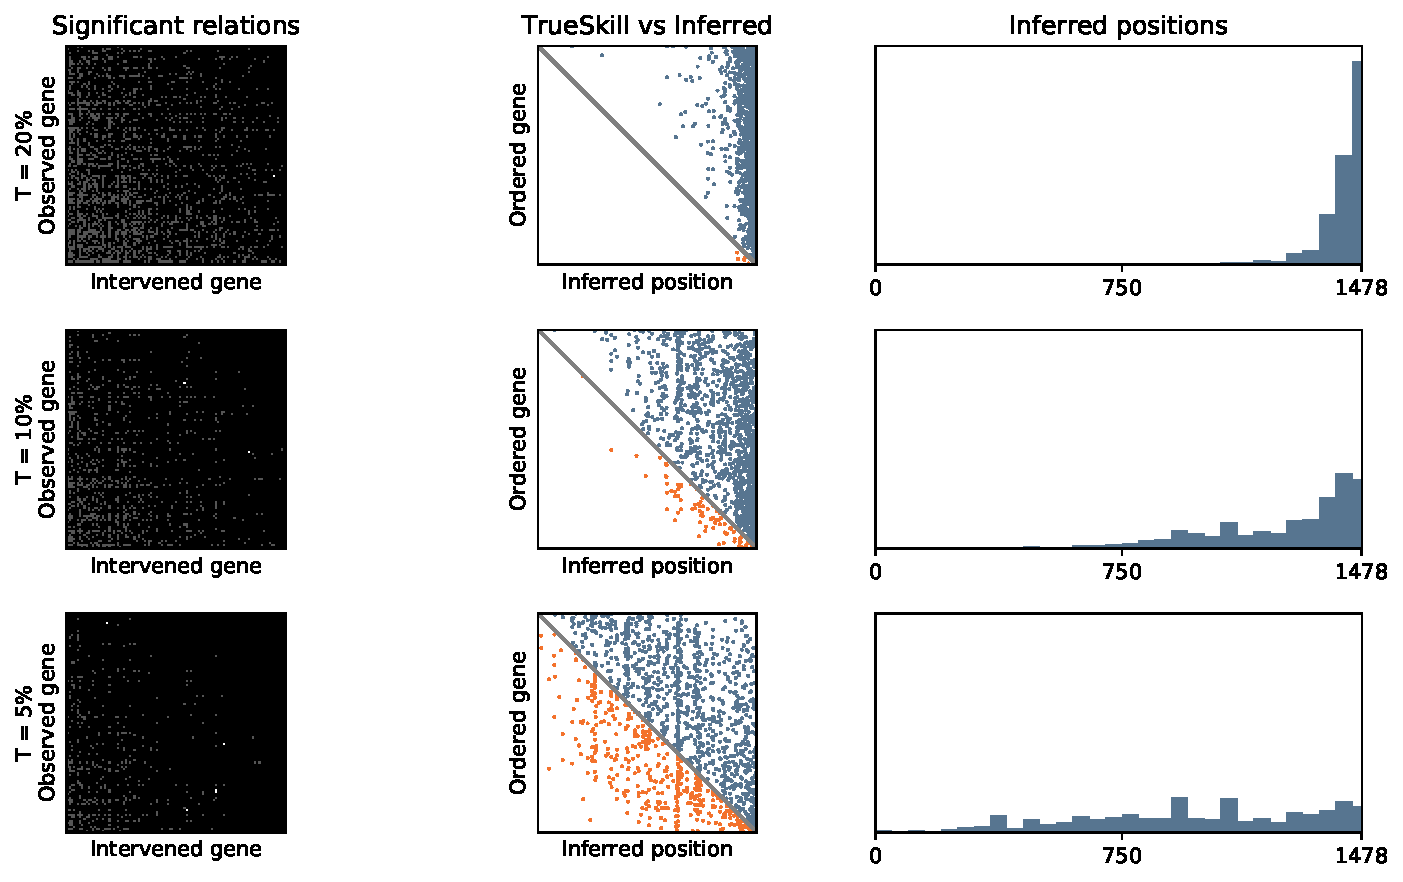
\includegraphics[width=\textwidth]{paper/5inferred_positions}
        \end{center}
    }
\end{frame}


% Come back to
\begin{frame}
    \frametitle{Order-Based LCD Algorithm}
    
    \only<1>{
        \begin{enumerate}
            \item \textbf{Order inference}: find an ancestral order of train variables \phantom{hallllllooooooooooooooo}
            \item \textbf{Position estimation}: find the position of a test variable in that order
            \item \textbf{Causal inference}: use LCD with an order-based $C$ to test causal relations
        \end{enumerate}
    }

    \only<2>{
        \begin{enumerate}
            \item \textbf{Order inference}: Sorted TrueSkill \phantom{halllllloooooooooooooooooooooooooooo}
            \item \textbf{Position estimation}: Simple conservative estimate \phantom{hallllllooooooooooooooo}
            \item \textbf{Causal inference}: Order-based LCD \phantom{hallllllooooooooooooooo}
        \end{enumerate}
    }


\end{frame}